% Options for packages loaded elsewhere
\PassOptionsToPackage{unicode}{hyperref}
\PassOptionsToPackage{hyphens}{url}
%
\documentclass[
]{book}
\usepackage{amsmath,amssymb}
\usepackage{lmodern}
\usepackage{iftex}
\ifPDFTeX
  \usepackage[T1]{fontenc}
  \usepackage[utf8]{inputenc}
  \usepackage{textcomp} % provide euro and other symbols
\else % if luatex or xetex
  \usepackage{unicode-math}
  \defaultfontfeatures{Scale=MatchLowercase}
  \defaultfontfeatures[\rmfamily]{Ligatures=TeX,Scale=1}
\fi
% Use upquote if available, for straight quotes in verbatim environments
\IfFileExists{upquote.sty}{\usepackage{upquote}}{}
\IfFileExists{microtype.sty}{% use microtype if available
  \usepackage[]{microtype}
  \UseMicrotypeSet[protrusion]{basicmath} % disable protrusion for tt fonts
}{}
\makeatletter
\@ifundefined{KOMAClassName}{% if non-KOMA class
  \IfFileExists{parskip.sty}{%
    \usepackage{parskip}
  }{% else
    \setlength{\parindent}{0pt}
    \setlength{\parskip}{6pt plus 2pt minus 1pt}}
}{% if KOMA class
  \KOMAoptions{parskip=half}}
\makeatother
\usepackage{xcolor}
\IfFileExists{xurl.sty}{\usepackage{xurl}}{} % add URL line breaks if available
\IfFileExists{bookmark.sty}{\usepackage{bookmark}}{\usepackage{hyperref}}
\hypersetup{
  pdftitle={S23 Summer School},
  pdfauthor={Caspar J. van Lissa¹ (only this GitBook; rest of the course by colleagues)},
  hidelinks,
  pdfcreator={LaTeX via pandoc}}
\urlstyle{same} % disable monospaced font for URLs
\usepackage{color}
\usepackage{fancyvrb}
\newcommand{\VerbBar}{|}
\newcommand{\VERB}{\Verb[commandchars=\\\{\}]}
\DefineVerbatimEnvironment{Highlighting}{Verbatim}{commandchars=\\\{\}}
% Add ',fontsize=\small' for more characters per line
\usepackage{framed}
\definecolor{shadecolor}{RGB}{248,248,248}
\newenvironment{Shaded}{\begin{snugshade}}{\end{snugshade}}
\newcommand{\AlertTok}[1]{\textcolor[rgb]{0.94,0.16,0.16}{#1}}
\newcommand{\AnnotationTok}[1]{\textcolor[rgb]{0.56,0.35,0.01}{\textbf{\textit{#1}}}}
\newcommand{\AttributeTok}[1]{\textcolor[rgb]{0.77,0.63,0.00}{#1}}
\newcommand{\BaseNTok}[1]{\textcolor[rgb]{0.00,0.00,0.81}{#1}}
\newcommand{\BuiltInTok}[1]{#1}
\newcommand{\CharTok}[1]{\textcolor[rgb]{0.31,0.60,0.02}{#1}}
\newcommand{\CommentTok}[1]{\textcolor[rgb]{0.56,0.35,0.01}{\textit{#1}}}
\newcommand{\CommentVarTok}[1]{\textcolor[rgb]{0.56,0.35,0.01}{\textbf{\textit{#1}}}}
\newcommand{\ConstantTok}[1]{\textcolor[rgb]{0.00,0.00,0.00}{#1}}
\newcommand{\ControlFlowTok}[1]{\textcolor[rgb]{0.13,0.29,0.53}{\textbf{#1}}}
\newcommand{\DataTypeTok}[1]{\textcolor[rgb]{0.13,0.29,0.53}{#1}}
\newcommand{\DecValTok}[1]{\textcolor[rgb]{0.00,0.00,0.81}{#1}}
\newcommand{\DocumentationTok}[1]{\textcolor[rgb]{0.56,0.35,0.01}{\textbf{\textit{#1}}}}
\newcommand{\ErrorTok}[1]{\textcolor[rgb]{0.64,0.00,0.00}{\textbf{#1}}}
\newcommand{\ExtensionTok}[1]{#1}
\newcommand{\FloatTok}[1]{\textcolor[rgb]{0.00,0.00,0.81}{#1}}
\newcommand{\FunctionTok}[1]{\textcolor[rgb]{0.00,0.00,0.00}{#1}}
\newcommand{\ImportTok}[1]{#1}
\newcommand{\InformationTok}[1]{\textcolor[rgb]{0.56,0.35,0.01}{\textbf{\textit{#1}}}}
\newcommand{\KeywordTok}[1]{\textcolor[rgb]{0.13,0.29,0.53}{\textbf{#1}}}
\newcommand{\NormalTok}[1]{#1}
\newcommand{\OperatorTok}[1]{\textcolor[rgb]{0.81,0.36,0.00}{\textbf{#1}}}
\newcommand{\OtherTok}[1]{\textcolor[rgb]{0.56,0.35,0.01}{#1}}
\newcommand{\PreprocessorTok}[1]{\textcolor[rgb]{0.56,0.35,0.01}{\textit{#1}}}
\newcommand{\RegionMarkerTok}[1]{#1}
\newcommand{\SpecialCharTok}[1]{\textcolor[rgb]{0.00,0.00,0.00}{#1}}
\newcommand{\SpecialStringTok}[1]{\textcolor[rgb]{0.31,0.60,0.02}{#1}}
\newcommand{\StringTok}[1]{\textcolor[rgb]{0.31,0.60,0.02}{#1}}
\newcommand{\VariableTok}[1]{\textcolor[rgb]{0.00,0.00,0.00}{#1}}
\newcommand{\VerbatimStringTok}[1]{\textcolor[rgb]{0.31,0.60,0.02}{#1}}
\newcommand{\WarningTok}[1]{\textcolor[rgb]{0.56,0.35,0.01}{\textbf{\textit{#1}}}}
\usepackage{longtable,booktabs,array}
\usepackage{calc} % for calculating minipage widths
% Correct order of tables after \paragraph or \subparagraph
\usepackage{etoolbox}
\makeatletter
\patchcmd\longtable{\par}{\if@noskipsec\mbox{}\fi\par}{}{}
\makeatother
% Allow footnotes in longtable head/foot
\IfFileExists{footnotehyper.sty}{\usepackage{footnotehyper}}{\usepackage{footnote}}
\makesavenoteenv{longtable}
\usepackage{graphicx}
\makeatletter
\def\maxwidth{\ifdim\Gin@nat@width>\linewidth\linewidth\else\Gin@nat@width\fi}
\def\maxheight{\ifdim\Gin@nat@height>\textheight\textheight\else\Gin@nat@height\fi}
\makeatother
% Scale images if necessary, so that they will not overflow the page
% margins by default, and it is still possible to overwrite the defaults
% using explicit options in \includegraphics[width, height, ...]{}
\setkeys{Gin}{width=\maxwidth,height=\maxheight,keepaspectratio}
% Set default figure placement to htbp
\makeatletter
\def\fps@figure{htbp}
\makeatother
\setlength{\emergencystretch}{3em} % prevent overfull lines
\providecommand{\tightlist}{%
  \setlength{\itemsep}{0pt}\setlength{\parskip}{0pt}}
\setcounter{secnumdepth}{5}
\usepackage{booktabs}
\usepackage{longtable}
\usepackage{array}
\usepackage{multirow}
\usepackage{wrapfig}
\usepackage{float}
\usepackage{colortbl}
\usepackage{pdflscape}
\usepackage{tabu}
\usepackage{threeparttable}
\usepackage{threeparttablex}
\usepackage[normalem]{ulem}
\usepackage{makecell}
\usepackage{xcolor}
\ifLuaTeX
  \usepackage{selnolig}  % disable illegal ligatures
\fi

\title{S23 Summer School}
\usepackage{etoolbox}
\makeatletter
\providecommand{\subtitle}[1]{% add subtitle to \maketitle
  \apptocmd{\@title}{\par {\large #1 \par}}{}{}
}
\makeatother
\subtitle{Advanced Course on using Mplus}
\author{Caspar J. van Lissa¹ (only this GitBook; rest of the course by colleagues)}
\date{¹Utrecht University, Methodology \& Statistics}

\begin{document}
\maketitle

{
\setcounter{tocdepth}{1}
\tableofcontents
}
\hypertarget{course}{%
\chapter*{Course}\label{course}}
\addcontentsline{toc}{chapter}{Course}

This course material is part of the \href{https://utrechtsummerschool.nl/courses/social-sciences/advanced-course-on-using-mplus}{Advanced Course on using Mplus},
a five-day summer school course hosted by Utrecht University's department of Methodology and Statistics. If you already know how to analyse your data in Mplus but want to learn more about what you are actually doing, and especially if you want to know more about advanced longitudinal analyses, this course is for you. The course consists of in-depth lectures on the fundamentals of Mplus and advanced longitudinal models.

\hypertarget{preparing-for-the-course}{%
\chapter{Preparing for the course}\label{preparing-for-the-course}}

This Chapter helps you prepare for the course. It shows how to install R and RStudio on your computer. We'll also provide some general information on R, and how you can get help if you get error messages.

If you're already using R, all of this might be nothing new for you. You may \textbf{skip} this chapter then.

If you have \textbf{never used R before, this Chapter is essential}, as it gives you some input on how R works, and how we can use it for our data analyses.

\hypertarget{installing-software}{%
\section{Installing software}\label{installing-software}}

If you use R on your own computer, you will need to install it yourself. You should first:

\begin{enumerate}
\def\labelenumi{\arabic{enumi}.}
\tightlist
\item
  Install R from \url{https://CRAN.R-project.org}
\item
  Install `RStudio' Desktop (Free) from \url{https://rstudio.com}
\end{enumerate}

\begin{center}\rule{0.5\linewidth}{0.5pt}\end{center}

\hypertarget{installpackages}{%
\subsection{Installing packages}\label{installpackages}}

As a prerequisite for this guide, you need to have a few essential \textbf{R packages} installed.

\begin{enumerate}
\def\labelenumi{\arabic{enumi}.}
\tightlist
\item
  Open RStudio
\item
  Inside RStudio, find the window named \textbf{Console} on the bottom left corner of your screen (it might fill the entire left side of the screen).
\item
  We will now install a few packages using R Code. Here's an overview of the packages, and why we need them:
\end{enumerate}

\begin{tabular}{l|l}
\hline
Package & Description\\
\hline
MplusAutomation & Control Mplus from R and parse model output\\
\hline
ggplot2 & A flexible and user-friendly plotting package\\
\hline
tidySEM & Plotting and tabulating the output of SEM-models\\
\hline
semTools & Comparing models, establishing measurement invariance across groups\\
\hline
\end{tabular}

To install these packages, we use the \texttt{install.packages()} function in R. One package after another, our code should look like this:

\begin{Shaded}
\begin{Highlighting}[]
\FunctionTok{install.packages}\NormalTok{(}\StringTok{"MplusAutomation"}\NormalTok{)}
\FunctionTok{install.packages}\NormalTok{(}\StringTok{"ggplot2"}\NormalTok{)}
\FunctionTok{install.packages}\NormalTok{(}\StringTok{"tidySEM"}\NormalTok{)}
\FunctionTok{install.packages}\NormalTok{(}\StringTok{"semTools"}\NormalTok{)}
\end{Highlighting}
\end{Shaded}

\hypertarget{get-started}{%
\subsection{Get started}\label{get-started}}

\hypertarget{starting-a-new-project-in-rstudio}{%
\subsection{Starting a new project in Rstudio}\label{starting-a-new-project-in-rstudio}}

To keep all your work organized, you should use a \textbf{project}. In Rstudio, click on the \emph{New project} button:

\includegraphics{tut_new_proj.png}

In the pop-up dialog, click \emph{New directory}, and again \emph{New project}.

type the desired directory name in the dialog (give it a meaningful name, e.g.~``TCSM\_course''), and use `Browse' if you need to change the directory where you store your projects. Now, in your project, click \emph{File \textgreater{} New file \textgreater{} R script}. This script file works just like notepad, or the syntax editor in SPSS: You type plain text, but you can run it any time you want. Conduct all of the exercises in this script file.

\hypertarget{code-conventions}{%
\subsection{Code conventions}\label{code-conventions}}

Throughout the guide, a consistent set of conventions is used to refer to code:

\begin{itemize}
\tightlist
\item
  Functions are in a code font and followed by parentheses, like
  \texttt{sum()} or \texttt{mean()}.
\item
  Other R objects (like data or function arguments) are in a code
  font, without parentheses, like \texttt{seTE} or \texttt{method.tau}.
\item
  Sometimes, we'll use the package name followed by two colons, like
  \texttt{lavaan::sem()}. This is valid R code and will run. The \texttt{lavaan::} part indicates that the function \texttt{sem()} comes from the package \texttt{lavaan}.
\end{itemize}

\hypertarget{getting-help}{%
\subsection{Getting Help}\label{getting-help}}

As you start to apply the techniques described in this guide to your data you will soon find questions that the guide does not answer. This section describes a few tips on how to get help.

\begin{enumerate}
\def\labelenumi{\arabic{enumi}.}
\tightlist
\item
  Every function in R has documentation (a help file). To see it, select the name of the function and press F1, or run the command \texttt{?} followed by the name of the function, e.g.: \texttt{?aov}. I have been using R for 10 years, and I still press F1 all the time to see how a function works.
\item
  If you get stuck, start with \textbf{Google}. Typically, adding ``R'' to a search is enough to restrict it to relevant results, e.g.: ``exploratory factor analysis R''. Google is particularly useful for error messages. If you get an error message and you have no idea what it means, try googling it. Chances are that someone else has been confused by it in the past, and there will be help somewhere on the web. (If the error message isn't in English,
  run \texttt{Sys.setenv(LANGUAGE\ =\ "en")} and re-run the code; you're
  more likely to find help for English error messages.)
\item
  If Google doesn't help, try \href{https://stackoverflow.com}{stackoverflow}. Start by spending a little time searching for an existing answer; including {[}R{]} restricts your search to questions and answers that use R.
\item
  Lastly, if you stumble upon an error (or typos!) in this guide's text or R syntax, feel free to contact \textbf{Caspar van Lissa} at \textbf{\href{mailto:c.j.vanlissa@uu.nl}{\nolinkurl{c.j.vanlissa@uu.nl}}}.
\end{enumerate}

\hypertarget{getting-the-course-data}{%
\section{Getting the course data}\label{getting-the-course-data}}

All of the course data files are available on a GitHub repository. You can download them all at once by going to \url{https://github.com/cjvanlissa/S23_student}, clicking the green button labeled `Code', and downloading a ZIP archive of the repository.

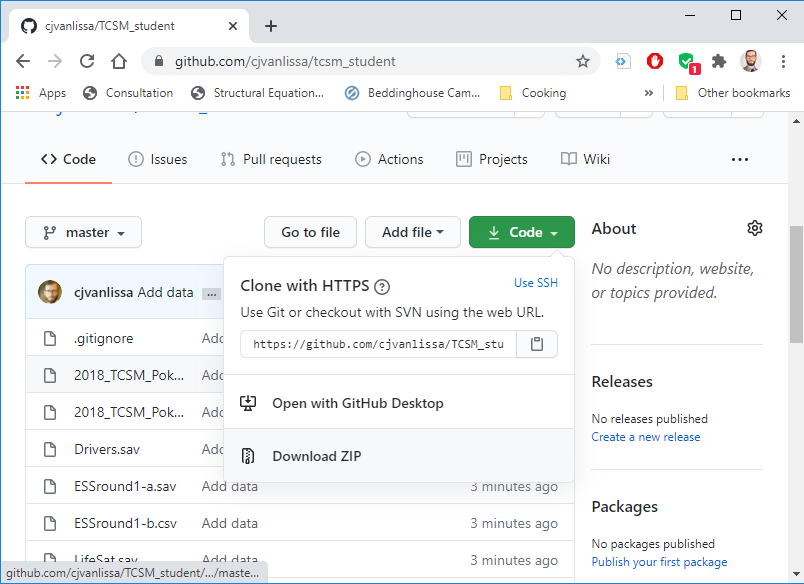
\includegraphics{coursematerials.png}

After unzipping the archive, you can open the RStudio project `S23\_student.Rproj', and the script `run\_me.R'. This script contains a few lines of code to help you install the required R-packages for the course.

\hypertarget{r-tutorial-for-beginners-optional}{%
\section{R tutorial for beginners (optional)}\label{r-tutorial-for-beginners-optional}}

Welcome to the world of R! This tutorial is based on the tutorial ``R: How to get started'' by \href{https://www.linkedin.com/in/ihnwhi-heo/}{Ihnwhi Heo}, \href{https://www.ducoveen.com/}{Duco Veen}, and \href{https://www.rensvandeschoot.com/}{Rens van de Schoot}, and adapted for TCSM.

\hypertarget{who-r-you}{%
\subsection{Who R you?}\label{who-r-you}}

R is\ldots{}

\begin{itemize}
\tightlist
\item
  Free programming software for statistical computation and graphics
\item
  Open source: everyone (even you!) can improve, develop, and contribute to R
\item
  The official manual by the R Core Team: \href{https://cran.r-project.org/doc/manuals/r-release/R-intro.pdf}{An introduction to R}
\end{itemize}

R itself looks a bit old-fashioned and tedious:

\includegraphics{tut_R.jpg}

\hypertarget{rstudio}{%
\subsection{RStudio}\label{rstudio}}

Thankfully, we have a great user interface for R, called RStudio!

\begin{itemize}
\tightlist
\item
  RStudio helps users to use and learn R easier
\item
  If you are using RStudio, this means you are using R.
\item
  From now on, all tutorials will go with RStudio.
\end{itemize}

\hypertarget{no-pane-no-gain}{%
\subsubsection{No `pane', no gain!}\label{no-pane-no-gain}}

When you open RStudio, the screen may look like this. You may notice that the screen is divided into A `panes' (a pane is a division of a window):

\includegraphics{tut_panes.jpg}

Before we explain these three panes - I want you to add the fourth one, which you will see if you open an R script. An R script is like a ``new document'' in Microsoft Word. When you open an R script, the fourth pane appears.

\hypertarget{create-a-new-r-script}{%
\subsubsection{Create a new R script}\label{create-a-new-r-script}}

Click the icon with a plus sign on the paper. Click the icon highlighted by the red square:

\includegraphics{tut_new_file.png}

When you click the icon, a new script appears in a fourth pane on the upper left side of the screen

\includegraphics{tut_panes2.jpg}

The four panes really help become organized. In RStudio, you can do everything all together on one screen. Thus, four panes make the work efficient (indeed, no `pain'!).

\hypertarget{what-do-the-four-panes-do}{%
\subsubsection{What do the four panes do?}\label{what-do-the-four-panes-do}}

\begin{itemize}
\tightlist
\item
  Out of four panes, the two on the left side are the panes you will use a lot.

  \begin{itemize}
  \tightlist
  \item
    Source pane: located at the top left side of the screen. It is also called the ``editor'', because this is where we edit scripts. We will usually type our code in the source pane.
  \item
    Console pane: located at the bottom left side of the screen. This panel is for direct communication with R. We can type commands here that are \emph{immediately} evaluated (whereas a script is only evaluated when we run it). Furthermore, all output of our commands is printed in this console pane.
  \end{itemize}
\item
  The panels on the right side of the screen contain various tabs. Among those tabs, it is worth looking at the Environment tab at the upper pane and the Plots tab at the lower pane.

  \begin{itemize}
  \tightlist
  \item
    The Environment tab contains all the `objects' currently loaded in your R session. In SPSS, you can have only one data file open. In R, you can have as many data `objects' as you like. They will be listed here. You can always check what objects are loaded under the environment tab. The environment is also called the `workspace'.
  \item
    The Plots tab shows various graphs and figures we draw. If you click Zoom with the magnifying glass, you can see plots in a bigger size.
  \end{itemize}
\end{itemize}

\hypertarget{day-2-latent-growth-curve-modeling-lgcm}{%
\chapter{Day 2: Latent growth curve modeling (LGCM)}\label{day-2-latent-growth-curve-modeling-lgcm}}

In this computer lab session you can practice with specifying latent growth models in Mplus and interpreting the output. All of the input files for the exercises described in this GitBook are provided with the course materials on SURFdrive.

\hypertarget{exercise-1-burn-survivors}{%
\section{Exercise 1: Burn survivors}\label{exercise-1-burn-survivors}}

The file \texttt{PTSD.dat} contains data on burn survivors, specifically:

\begin{itemize}
\tightlist
\item
  gender (\texttt{gender}),
\item
  percentage total body surface burned (\texttt{tvlo}),
\item
  SVL at wave 1 (2 weeks after burn injury; \texttt{W1}),
\item
  SVL at wave 2 (4 weeks after burn injury; \texttt{W2}),
\item
  SVL at wave 3 (2 months after burn injury; \texttt{W3}),
\item
  SVL at wave 4 (4 months after burn injury; \texttt{W4}),
\item
  SVL at wave 5 (6 months after burn injury; \texttt{W5}),
\item
  SVL at wave 6 (9 months after burn injury; \texttt{W6}),
\item
  SVL at wave 7 (12 months after burn injury; \texttt{W7}),
\item
  SVL at wave 8 (18 months after burn injury; \texttt{W8}), and
\item
  BPAS at wave 9 (24 months after burn injury; \texttt{pain}),
\end{itemize}

in this order.

\hypertarget{exercise-1a-specifying-a-lgcm}{%
\subsection{Exercise 1a: Specifying a LGCM}\label{exercise-1a-specifying-a-lgcm}}

Specify a latent growth curve model. Consider different specifications discussed in the lecture, and try to find the best specification. Use only the time measurements, not including additional predictor variables. Think about which metric of time to use and the shape of the function (linear or quadratic). Base your decision of the best model on plots (!), model fit indices, model comparison tools, and interpretation of the model parameters.

If you have reason to believe that another type of LGCM fits the data better, feel free to specific and estimate that model.

Click to show answers

\textbf{Deciding on the metric of time}

Based on these descriptions, I've chosen for the following specification of time in the LGM:

\texttt{i\ s\ \textbar{}\ W1@0.5\ W2@1\ W3@2\ W4@4\ W5@6\ W6@9\ W7@12\ W8@18;}

In this specification I set the first time point to 0.5 months after burn injury (approximation of 2 weeks after burn injury), the second time point to 1 month after burn injury (approximation of 4 weeks after burn injury), etc.

\textbf{Plots}
You can enable the plot functionality of Mplus by specifying

\begin{verbatim}
PLOT:
  TYPE = PLOT3;
  SERIES = W1 W2 W3 W4 W5 W6 W7 W8 (s);
\end{verbatim}

The \texttt{TYPE\ =\ PLOT3;} function ensures that all kinds of different types of plots are available in Mplus (see the Mplus User Guide for an overview of the different types of plots). The \texttt{SERIES\ =\ ...;} function tells Mplus to draw a line through the named variables in that order, for each individual.

EXPLAIN HOW TO GET NATIVE PLOTS OF MPLUS AND SHOW THEM HERE.

\textbf{Deciding on linear vs.~linear and quadratic slope}

Some example syntaxes for running models with different trajectory shapes are available in SURFdrive. These include:

\begin{enumerate}
\def\labelenumi{\arabic{enumi}.}
\tightlist
\item
  A LGCM with only a linear slope.
\item
  A LGCM with an added quadratic slope.
\item
  A LGCM with an added quadratic slope but no quadratic slope factor variance.
\end{enumerate}

For the model with a quadratic slope, it was necessary to fix the variance of Q at 0 to ensure convergence. For both models, only CFI and TLI indicate adequate fit.

\begin{longtable}[]{@{}
  >{\raggedright\arraybackslash}p{(\columnwidth - 14\tabcolsep) * \real{0.1967}}
  >{\centering\arraybackslash}p{(\columnwidth - 14\tabcolsep) * \real{0.1967}}
  >{\centering\arraybackslash}p{(\columnwidth - 14\tabcolsep) * \real{0.1148}}
  >{\centering\arraybackslash}p{(\columnwidth - 14\tabcolsep) * \real{0.1148}}
  >{\centering\arraybackslash}p{(\columnwidth - 14\tabcolsep) * \real{0.1148}}
  >{\centering\arraybackslash}p{(\columnwidth - 14\tabcolsep) * \real{0.0820}}
  >{\centering\arraybackslash}p{(\columnwidth - 14\tabcolsep) * \real{0.0820}}
  >{\centering\arraybackslash}p{(\columnwidth - 14\tabcolsep) * \real{0.0984}}@{}}
\toprule
\begin{minipage}[b]{\linewidth}\raggedright
Model
\end{minipage} & \begin{minipage}[b]{\linewidth}\centering
Parameters
\end{minipage} & \begin{minipage}[b]{\linewidth}\centering
AIC
\end{minipage} & \begin{minipage}[b]{\linewidth}\centering
BIC
\end{minipage} & \begin{minipage}[b]{\linewidth}\centering
RMSEA
\end{minipage} & \begin{minipage}[b]{\linewidth}\centering
CFI
\end{minipage} & \begin{minipage}[b]{\linewidth}\centering
TLI
\end{minipage} & \begin{minipage}[b]{\linewidth}\centering
SRMR
\end{minipage} \\
\midrule
\endhead
exercise1a.out & 13 & 14051 & 14096 & .14 & .93 & .94 & .08 \\
exercise1a\_Q.out & - & - & - & - & - & - & - \\
exercise1a\_Q0.out & 14 & 14037 & 14085 & .13 & .94 & .94 & .08 \\
\bottomrule
\end{longtable}

\textbf{Model comparison tools}

To see which model fit the data better, we can do a \(\Delta \chi^{2}\) (i.e., Chi-square difference) test (e.g., using the function \texttt{chisq\_sb()} from the \texttt{tidySEM} package in R, or using on online \(\chi^{2} calculator\)): \(\Delta \chi^{2} = 16.14\), \(\Delta df = 1\), \(p < .001\). Furthermore, both AIC and BIC are lower in the model with a quadratic slope. Thus, model misfit is significantly lower when the quadratic slope is added although the fit indices still do not indicate adequate fit. We can use the plots, \texttt{RES} option in Mplus, or modification indices to see what the source of the misfit is.

\textbf{Model parameters}

The mean of the quadratic slope factor is significant (\texttt{q\ =\ 0.02}, \(p < .001\)), indicating that, on average, the growth curve does follow a quadratic curve (see \texttt{exercise1a\_Q0.out}).

\hypertarget{exercise-1b-adding-covariates}{%
\subsection{Exercise 1b: Adding covariates}\label{exercise-1b-adding-covariates}}

Using the best fitting LGM model found above, regress the growth parameters on \texttt{TVLO} and regress \texttt{pain} on the growth components. Then investigate if there are gender differences in the regression of the growth parameters on \texttt{TVLO} and in the regression of \texttt{pain} on the growth parameters?

Click to show answers

Rephrasing the question, we are asked to investigate if gender moderates the predictive relationship of \texttt{TVLO} on the growth components, as well as the relationship between the growth components and \texttt{Pain}. As such, we can do a multigroup analysis by gender, resulting in the addition of the following syntax to the \texttt{VARIABLE:} command:

\texttt{GROUPING\ =\ gender\ (1\ =\ male\ 2\ =\ female);}

Since we needed to fix the quadratic slope variance to 0, we cannot estimate any regressions on the quadratic slope or use the quadratic slope as a predictor of some outcome. We therefore focus on the intercept and linear slope.

The file \texttt{exercise1B.inp} on SURFdrive contains the Mplus syntax on how to specify this model, including the \texttt{MODEL\ TEST} command to test between-group (i.e., between-gender) differences in the effect of \texttt{TVLO} on the growth components, and the growth components on \texttt{pain}. This is only an illustrative example for how to approach this analysis; your specific execution may differ (e.g., you could specify 2 models, and with across group constraints and one without, and then use the \(\Delta \chi^{2}\) test to see if the improvement of model fit is significant). Note that in this example, the Wald \(\chi^2\) p-value is not significant. That means that there are no significant gender differences in the effect of the growth trajectory on pain.

Note that the Wald test is an overall test of \textbf{all} comparisons that we specify in \texttt{MODEL\ TEST}. Thus, if you want a separate test for the regression of TVLO on the growth parameters, you need to re-run the analysis but with a different \texttt{MODEL\ TEST} argument.

Conclusion: There are no gender differences in the regression of growth parameters on TVLO and in the regression of Pain on the growth parameters.

\hypertarget{exercise-2-alcohol-use}{%
\section{Exercise 2: Alcohol use}\label{exercise-2-alcohol-use}}

The figure below depicts the basic LGCM for the alcohol use data from Duncan, Duncan, and Strycker (2006), example 8\_1.

\begin{figure}
\centering
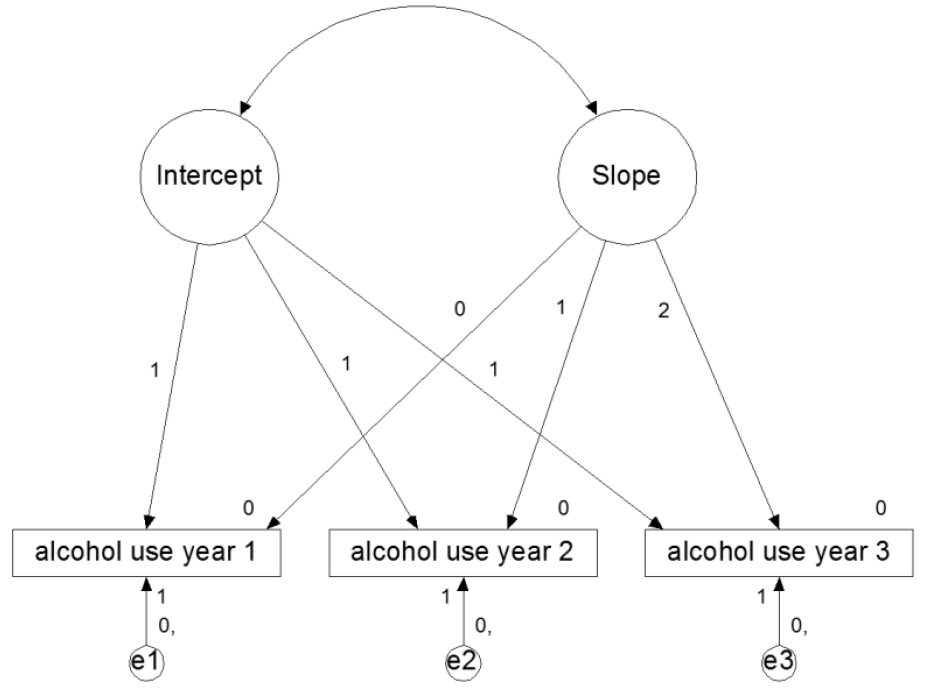
\includegraphics[width=4.16667in,height=\textheight]{./figures/Duncan-LGCM.png}
\caption{Latent growth curve model for alcohol use.}
\end{figure}

The data are in the file \texttt{DDS8\_1.dat}, with variables \texttt{ALC1YR1} \texttt{ALC1YR2} \texttt{ALC1YR3} \texttt{ALCPROB5} \texttt{AGE1} and \texttt{GENDER1} (in that order). Missing values are coded as \texttt{-99}. The variable \texttt{ALCPROB5} is categorical, it indicates alcohol problems in year 5 of the study (0 = no, 1 = yes).

\hypertarget{exercise-2a-specify-a-lgcm}{%
\subsection{Exercise 2a: Specify a LGCM}\label{exercise-2a-specify-a-lgcm}}

Set up the LGCM as depicted in the figure above in Mplus using the \texttt{\textbar{}} notation (rather than specifying a CFA by using the \texttt{BY} statement). Inspect the output carefully with special attention for a) the pattern of missing values, b) the model fit, and c) the interpretation of the parameter estimates. How well does the model predict alcohol use of the years?

Click to show answers

The input and output file (\texttt{exercise2A.inp} and \texttt{exercise2A.out}) can be found on SURFdrive. The table under \texttt{PROPORTION\ OF\ DATA\ PRESENT} in the output file shows that the majority of the cases is complete, but that there is a small amount of attrition (panel dropout). You can also inspect the coverage matrix to inspect how much information you have for different parts of the model. Regarding model fit, the model fits well overall with the chi-square test of model fit \(\chi^{2}(1) = 2.781\), \(p = 0.095\), and the CFI and TLI above their recommended cutoff points. However, the RMSEA implies some some degree of misfit at \(0.062\). The intercept and slope means indicate a relatively high starting point (3.68, \(SE = .081\)) and a growth of 0.92 (\(SE = .053\)) per year. The intercept and slope factors show considerable variance, indicating that the starting points and rates of growth differ considerably across individuals. Interestingly, the explained variance \(R^{2}\) is high for years 1 and 3, but lower for year 2.

\hypertarget{exercise-2b-predicting-growth}{%
\subsection{Exercise 2b: Predicting growth}\label{exercise-2b-predicting-growth}}

We will now \emph{explore} how different predictor variables affect the model fit. Include gender and age in the model as predictors of the intercept and slope. Interpret the fit of the model and the output. Feel free to estimate several models, including or excluding certain covariates. Make a model fit table by hand in a spreadsheet, reporting on the fit indices you deem to be appropriate. Which model do you consider to be best?

\hypertarget{exploratory-vs-confirmatory-research}{%
\subsubsection{Exploratory vs confirmatory research}\label{exploratory-vs-confirmatory-research}}

Note that when you conduct \emph{confirmatory} research, and are testing theoretical hypotheses, you should not add and omit paths based on exploratory analyses and model fit. It is fine to add and remove paths in \emph{exploratory} research. Model fit indices, like AIC and BIC, are suitable for selecting well-fitting models in exploratory research. p-values are not designed for variable selection, and using them for that purpose may lead to sub-optimal models.

It is good scientific practice to clearly separate confirmatory and exploratory research. When you conduct exploratory research, you should not perform inference on the resulting parameters based on p-values (because inference generalizes your findings to the population, and exploratory findings tend to be tailored toward this specific sample). You should also not present exploratory results as if they were testing a post-hoc theory (also referred to as ``Hypothesizing After the Results are Known'', or \emph{HARKing}). This is a questionable research practice and can lead to false-positive (spurious) findings.

Click to show answers

The files \texttt{exercise2B\_M1.inp}, \texttt{exercise2B\_M2.inp}, and \texttt{exercise2B\_M3.inp}, on SURFdrive contain various models in which we predict the growth components using \texttt{AGE1} and \texttt{GENDER1}. The model fit remains excellent. After removing non-significant paths from \texttt{exercise2B\_M1.inp} (order based on magnitude of standardized effect size), gender and age only predict the starting point but not the slope. However, after having removed the effect of gender and age on the slope, the model suddenly fits very badly (\texttt{exercise2B\_M2.inp}). Careful inspection of the output shows that the covariance between intercept and slope has disappeared from the model (it is now the covariance between a latent variable and a residual, Mplus automatically puts these at zero). Mplus automatically constrains these to zero. If we add the statement \texttt{I\ WITH\ S} to the model, we obtain a good fit with significant effects of both gender and age on the intercept (\texttt{exercise2B\_M3.inp}). This illustrates the importance of checking the output carefully to find out if Mplus is actually doing what you think it does!

\hypertarget{exercise-2c-categorical-distal-outcome}{%
\subsection{Exercise 2c: Categorical distal outcome}\label{exercise-2c-categorical-distal-outcome}}

Include alcohol problems in year 5 in the model. Let the intercept and slope factors predict alcohol problems in year 5. Declare the variable as categorical in the variable section (\texttt{CATEGORICAL\ =\ ALCPROB5}). Inspect if the effect of age and gender on alcohol problems year 5 is completely mediated by the growth factors, or if there are additional direct paths from age and gender on the alcohol problems.

Click to show answers

The model fit is still good. Note that after adding a categorical dependent variable to the model, Mplus switches to a robust estimator (MLR, and the exact type of regression the Mplus uses now is a logit regression). Both intercept and slope predict alcohol problems (see \texttt{exercise2c\_M1.inp} on SURFdrive). Age also predicts alcohol problems directly (see \texttt{exercise2c\_M2.inp} on SURFdrive). Since age predicts alcohol problems both directly and via the intercept, a mediation analysis is in order. This shows that the indirect effect of age via the intercept on alcohol problems is still significant when the direct effect is added to the model.

\hypertarget{exercise-3-level-and-shape-parameterization}{%
\section{Exercise 3: Level and shape parameterization}\label{exercise-3-level-and-shape-parameterization}}

The file \texttt{GPA.dat} holds the following variables (in that order):

\begin{itemize}
\tightlist
\item
  grade point average (GPA) data with GPA scores of 200 students in 6 consecutive semesters (\texttt{gpa1}, \ldots, \texttt{gpa6})
\item
  high school GPA \texttt{highpa}
\item
  gender \texttt{sex}
\item
  admitted to university of choice (missing if not applied for university, \texttt{student})
\end{itemize}

In this exercise you will use the GPA data to set up a level and shape model (i.e., a LGCM with estimated time scores).

\hypertarget{exercise-3a}{%
\subsection{Exercise 3a}\label{exercise-3a}}

Use a parameterization with \texttt{GPA1@0} and \texttt{GPA6@1}. The loadings for the other time points should be freely estimated. This can be done with, for example, the syntax \texttt{GPA2*} as shown in the handout. Interpret the factor loadings and estimate for \texttt{S}.

Click to show answers

The Mplus model syntax for this LGCM can be found in \texttt{exercise3A.inp} on SURFdrive. The factor loadings indicate the proportion of change for a 1 unit change in time (here, a 1 unit change of time is specified as the change between the first and the last time points). The predicted change in the outcome for a 1 unit change in time is the mean of the slope, \(\alpha_{S} = 0.55\). Therefore, when looking at the factor loadings, 24\% of the total change occurs between \texttt{GPA1} and \texttt{GPA2.}. The intercept at \texttt{GPA1} = 2.575. So the estimated score at \texttt{GPA2} is \(GPA1 = 2.575 + 0.239*0.549 = 2.706\). The estimated score at \texttt{GPA3} is \(GPA3 = 2.575 + 0.450*0.549 = 2.822\), etc.

\hypertarget{exercise-3b}{%
\subsection{Exercise 3b}\label{exercise-3b}}

Now use a parameterization with \texttt{GPA1@0} and \texttt{GPA2@1}. The other GPA's should be freely estimated. Interpret the factor loadings and estimate for S.

Click to show answers

The Mplus model syntax for this parametrization of the LGCM with freely estimated time scores can be found in \texttt{exercise3B.inp}. The mean of the slope factor \(\alpha_{S}\) now indicates the difference between \texttt{GPA1} and \texttt{GPA2}. The estimated factor loadings indicate the distance in units from the starting point, where 1 unit is S. In other words, every distance compares to the increase between GPA1 and GPA2.

Which parameterization do you like best?

\hypertarget{exercise-3c}{%
\subsection{Exercise 3c}\label{exercise-3c}}

Draw the development of GPA over time, using the parametrization of your choice) based on your own calculations (by hand). Compare this to the estimated means plot that you can get with the plot command:

\begin{verbatim}
PLOT: 
  SERIES = GPA1-GPA6 (s); 
  TYPE = PLOT3;
\end{verbatim}

Don't forget that you need to rescale that plot, since \texttt{S} is linear while the location of the estimated points is based on the factor loadings.

Click to show answers

The estimated means plot for the parametrization (0 1 * * * *) is shown below, and can be generated by clicking the plots button, and selecting ``Estimated means''.

\begin{figure}
\centering
\includegraphics[width=4.16667in,height=\textheight]{./figures/exercise3C-estimatedMeans.jpg}
\caption{Estimated means}
\end{figure}

\hypertarget{exercise-3d}{%
\subsection{Exercise 3d}\label{exercise-3d}}

Use sex as a predictor of the intercept and slope and interpret the result (with 0 = boys, 1 = girls).

Click to show answers

The Mplus model syntax for the LGCM with time scores (0 * * * * 1) and gender predicting the growth components can be found in \texttt{exercise3D.inp}. Sex is a significant predictor of the intercept and a significant predictor of development, with girls having a higher initial level (\(b = .079\), \(SE = .037\)), and a greater development over time (\(b = .136\), \(SE = .054\)). Who run the world?

\hypertarget{exercise-4-latent-growth-curve-model-on-gpa-data}{%
\section{Exercise 4: Latent growth curve model on GPA data}\label{exercise-4-latent-growth-curve-model-on-gpa-data}}

\hypertarget{exercise-4a}{%
\subsection{Exercise 4a}\label{exercise-4a}}

Continuing with the data used for the previous exercise, set up a latent growth model for GPA for the 6 consecutive occasions and run this model. Obtain the following parameters:

\begin{itemize}
\tightlist
\item
  AIC, BIC, \(\chi^{2}\), RMSEA, CFI, and TLI;
\item
  The mean of the intercept factor \(\alpha_{I}\) and slope factor \(\alpha_{S}\);
\item
  The variance of the intercept facor \(\psi_{I}\) and slope factor \(\psi_{S}\).
\end{itemize}

Click to show answers

The Mplus model syntax for this can be found in \texttt{exercise4A.inp}.

\hypertarget{exercise-4b}{%
\subsection{Exercise 4b}\label{exercise-4b}}

Then, set up a latent growth curve model for 3 years where each year is a latent variable measured by the GPA of two consecutive semesters.

The factor loadings for GPA2, GPA4 and GPA6 ought to be constrained to be equal with a label (a) behind the loading in the syntax. As such, the scores relate in the same way to the year score over time. The GPA intercepts are constrained at 0.

If you get the error message below, can you find out what the problem is?

\begin{verbatim}
WARNING:  THE LATENT VARIABLE COVARIANCE MATRIX (PSI) IS NOT POSITIVE DEFINITE. THIS 
COULD INDICATE A NEGATIVE VARIANCE/RESIDUAL VARIANCE FOR A LATENT VARIABLE, A CORRELATION 
GREATER OR EQUAL TO ONE BETWEEN TWO LATENT VARIABLES, OR A LINEAR DEPENDENCY AMONG MORE 
THAN TWO LATENT VARIABLES. CHECK THE TECH4 OUTPUT FOR MORE INFORMATION. 
\end{verbatim}

A rough way to deal with this problem may be to fix the problematic parameter to a particular value (e.g., .001), try this and rerun the model. Now examine the same parameters as for exercise 4a, and compare the two. Are there major differences?

Click to show answers

The Mplus model syntax for this can be found in \texttt{exercise4B\_M2.inp}. Note that, without \texttt{year3@.001} (see \texttt{exercise4B\_M1.inp}), this code gives an error message: The variance of the latent variable year3 is estimated negatively which is problematic since variances should always be positive. A simple way to deal with the problem of the latent variance of year3 is to fix it to a very small value (.001) for instance, as it would also be illogical to fix a variance to 0. To do this, simply add this to your input file under model: \texttt{year3@.001;}

If you inspect the output carefully (and provided you have requested standardized estimates) you will notice that the latent variables \texttt{year2} and \texttt{year3} have a correlation of 1. So the negative variance is the result of a multicolinearity problem. It is apparently better to analyze these data using only the observed variables \texttt{gpa1-gpa6}. Creating latent variables per year does not work well. In line with this interpretation, the fit and results of the simple latent growth model look better than the 2nd order latent growth curve model.

\hypertarget{day-3-longitudinal-mixture-modeling}{%
\chapter{Day 3: Longitudinal mixture modeling}\label{day-3-longitudinal-mixture-modeling}}

The exercises in this lab session are designed, in the first place, for use of Mplus exclusively. However, for those interested, we have the option to run the latent growth mixture models in batch, using the R-package \texttt{MplusAutomation}. This package allows you to automate part of your workflow (like making plots and tables), and provides functions for plots that are, and now I'm politically correct, more aesthetically pleasing, as well as more insightful. The exercises using \texttt{MplusAutomation} can be found with the course materials on SURFdrive.

All of the input files using Mplus that I refer to in these exercises are provided with the course material on SURFdrive.

\hypertarget{exercise-1-latent-growth-mixture-modeling}{%
\section{Exercise 1: Latent growth (mixture) modeling}\label{exercise-1-latent-growth-mixture-modeling}}

The goal of this exercise is to subpopulations with different alcohol use trajectories. To this end, we start with an exploratory latent class growth analysis, and work towards a growth mixture model.

\hypertarget{exercise-1a-exploratory-lcga}{%
\subsection{Exercise 1a: Exploratory LCGA}\label{exercise-1a-exploratory-lcga}}

First, we perform an exploratory latent class growth analysis (LCGA) as initial exploratory option. Set up LCGA models models for 1, 2, 3, and 4 classes for the data in \texttt{DDS8\_1.dat}. Specify the model using the \texttt{\textbar{}} notation, and constrain the variances of the intercept and slope factors to be equal to 0. Furthermore, request \texttt{TECH11}, and \texttt{TECH14} to help evaluate model fit.

Click to show answers

Mplus model syntax for the LCGA models for 1, 2, 3, and 4 classes are in \texttt{exercise1A\_1C.inp}, \texttt{exercise1A\_2C.inp}, \texttt{exercise1A\_3C.inp}, \texttt{exercise1A\_4C.inp}, respectively.

\hypertarget{exercise-1b}{%
\subsection{Exercise 1b}\label{exercise-1b}}

These models use random starting values. Several independent random starts are made, to ensure that the model converges on the proper solution. The default is 20 random sets of starting values, of which 4 are run to completion. Inspect the output, and look carefully if the model estimation has converged, especially for the larger number of classes. Look for warning and error messages, make sure you understand what they are telling you.

The \texttt{STARTS} option is used to specify the number of initial random starting values and final stage optimizations. Now, increase the number of starts to ensure proper convergence. Once you are confident that the model has converged to the proper solution, compare the different models using the available fit information (e.g., BIC, LMR-LRT, BLRT, entropy, min. N in classes, etc.). Which model do you prefer, and why?

Click to show answers

You can inspect the convergence of the model by checking that the best final state loglikelihood value has been replicated using different starting values. See the output section \texttt{RANDOM\ STARTS\ RESULTS\ RANKED\ FROM\ THE\ BEST\ TO\ THE\ WORST\ LOGLIKELIHOOD\ VALUES}. Increasing the number of random starts can be done by specifying \texttt{STARTS\ =\ 50\ 10;} in the \texttt{ANALYSIS} command, where the first number specifies the initial number of random starts, and the second number specifies the number of initial starts that will be converged to the final stage.

Based on the fit indices of the fitted LCGA models, I would select a 3-class model. The fit indices and (LMR-LRT tests essentially indicate that you can keep adding classes and improve the model, which makes it difficult to decide. However, if we look at the counts in each class, we see that from 4 classes onward, the smallest class has less than 10\% of cases assigned to it. The minimum posterior classification probability and entropy are best for the 3-class model, which means that this model can reasonably accurately assign individuals to classes.

\hypertarget{exercise-1c-growth-mixture-models}{%
\subsection{Exercise 1c: Growth mixture models}\label{exercise-1c-growth-mixture-models}}

Set up the same models as analyzed in the previous exercise, but now allow the means and variances of the intercept and slope factors to be freely estimated in each class (i.e., a growth mixture model). You do this by mentioning the intercept and slope explicitly in the class-specific part of the syntax. This is a more complex model, and we might therefore expect that we will need fewer classes for a good description of the data. This analysis will also take more computing time, so add \texttt{PROCESSORS\ =\ 4} to the analysis section. Make a table of the fit indices, look at BIC, the LMR-LRT (\texttt{TECH11}), and the bootstrapped LRT value (\texttt{TECH14}).

Click to show answers

Mplus model syntax for the GMM models for 1, 2, 3, and 4 classes are in \texttt{exercise1C\_1C.inp}, \texttt{exercise1C\_2C.inp}, \texttt{exercise1C\_3C.inp}, \texttt{exercise1C\_4C.inp}, respectively. The BLRT for the GMM with 3 classes warns that \texttt{OF\ THE\ 10\ BOOTSTRAP\ DRAWS,\ 7\ DRAWS\ HAD\ BOTH\ A\ SMALLER\ LRT\ VALUE\ THAN\ THE\ OBSERVED\ LRT\ VALUE\ AND\ NOT\ A\ REPLICATED\ BEST\ LOGLIKELIHOOD\ VALUE\ FOR\ THE\ 3-CLASS\ MODEL.} You can increase the number of random starts for the BLRT using \texttt{LRTSTARTS\ =\ 0\ 0\ 40\ 10;} in the \texttt{ANALYSIS} command. Also note the convergence problems for the GMM with 4 classes. This indicates that a model with 4 classes is likely to be too complex for the data. Furthermore, since the GMM with only a single class is equivalent to a ``simple'' LGCM, we focus on the GMM with 2 and 3 classes in the next exercises.

\hypertarget{exercise-1d-model-predicted-trajectory-plots}{%
\subsection{Exercise 1d: Model-predicted trajectory plots}\label{exercise-1d-model-predicted-trajectory-plots}}

Plotting the model-predicted trajectories makes it easier to interpret the model. Moreover, visualizing the raw data provides yet another way to evaluate the fit of your mixture model to the data. With this in mind, plot the GMM models with 2 and 3 classes you created in exercise 1c, and interpret what you see. First, plot only the predicted trajectories. Then, plot raw data as well. Explain the benefit of plotting the raw data in your own words.

Click to show answers

Plotting the raw data helps us understand how representative the average trajectory for each class captures the individual trajectories of individuals in that class. It helps us see how separable the classes are visually, instead of just relying on statistics like entropy. To get plots, make sure you include:

\begin{verbatim}
PLOT:
    TYPE = PLOT3;
    SERIES = ALC1YR1(1) ALC1YR2(2) ALC1YR3(3);
\end{verbatim}

when running the model. Then press the ``plot'' button and select ``Estimated mean and observed individual values'' and ``Estimated means and estimated individual values''. Below you can find these plots for the GMM with 2 classes.

\begin{figure}
\centering
\includegraphics[width=4.16667in,height=\textheight]{./figures/exercise1D-estimatedMeansIndividualValues.jpg}
\caption{Estimated means and individual values.}
\end{figure}

\begin{figure}
\centering
\includegraphics[width=4.16667in,height=\textheight]{./figures/exercise1D-estimatedMeansAndValues.jpg}
\caption{Estimated means and estimated invidivual trajectories}
\end{figure}

Admittedly, this plot looks chaotic. Primarily because the individual values are not colored according to the class to which they are assigned. Alternatively, you could get the estimated means and (individual) values per class in a seperate window as well. However, \texttt{MplusAutomation} has some useful plotting functions that I recommend you to explore, for example \texttt{plotGrowthMixtures()}, in which you can color the lines according to their class membership.

\hypertarget{exercise-1e}{%
\subsection{Exercise 1e}\label{exercise-1e}}

Covariates are often added to mixture models, to predict 1) class membership 2) to explain variation in the growth parameters within the classes, or 3) as a distal outcome. Whenever covariates are however added to the model, they change the latent class solution. Sometimes, this is fine, as the covariates can help to improve the classification. In other cases, you would use a 3-step approach, which Mplus has automated:

\begin{enumerate}
\def\labelenumi{\arabic{enumi}.}
\tightlist
\item
  Fit an unconditional LCA (without covariates).
\item
  A ``most likely class variable'' is created using the posterior distribution of step 1.
\item
  This most likely class variable is then regressed on (a) covariate.
\end{enumerate}

There are a few options for how to do 3-step analysis. They all rely on adding to the \texttt{VARIABLE} command. For more info, see \url{https://www.statmodel.com/download/webnotes/webnote15.pdf}.

\hypertarget{commands-for-conducting-a-3-step-model}{%
\subsubsection{Commands for conducting a 3-step model}\label{commands-for-conducting-a-3-step-model}}

You can add the following options to the \texttt{VARIABLE} command:

\begin{enumerate}
\def\labelenumi{\arabic{enumi}.}
\tightlist
\item
  \texttt{AUXILIARY\ =\ x(R)}\strut \\
  This is actually a 1-step method for predicting latent class memberships using Pseudo-Class draws.
\item
  \texttt{AUXILIARY\ =\ x(R3step);}\strut \\
  A 3-step procedure, where covariates predict the latent class.
\item
  \texttt{AUXILIARY\ =\ y(e)}\strut \\
  A 1-step method, where the latent class predicts a continuous distal outcome.
\item
  \texttt{AUXILIARY\ =\ y(de3step);}\strut \\
  A 3-step procedure, where latent class predicts continuous covariates (distal outcome) with unequal means and equal variances.
\item
  \texttt{AUXILIARY\ =\ y(du3step);}\strut \\
  A 3-step procedure, where latent class predicts continuous covariates (distal outcome) with unequal means and variances.
\item
  \texttt{AUXILIARY\ =\ Y(dcon);}\strut \\
  Procedure for continuous distal outcomes as suggested by Lanza et al (2013).
\item
  \texttt{AUXILIARY\ =\ Y(dcon);}\strut \\
  Procedure for categorical distal outcomes as suggested by Lanza et al (2013).
\item
  \texttt{AUXILIARY\ =\ y(BCH);}\strut \\
  Improved and currently best 3-step procedure with continuous covariates as distal outcomes.
\end{enumerate}

Pick your final model from 1c, and add both age and gender as auxiliary variables in the model. Try to think what 3-step model you want, and if you are not sure, run different models, so you can evaluate how the different procedures make a difference. What is the effect of both age and gender?

Click to show answers

I'm providing an example using the 3-step procedure in \texttt{exercise1E.inp}. The results of adding these covariate to the model as predictors of the latent class can be found under the heading \texttt{TESTS\ OF\ CATEGORICAL\ LATENT\ VARIABLE\ MULTINOMIAL\ LOGISTIC\ REGRESSIONS\ USING\ THE\ 3-STEP\ PROCEDURE}. It can be seen, from the overall test and the pairwise comparisons, that the third group is significantly older, and has a significantly lower proportion of girls than the other two classes.

\hypertarget{exercise-2-latent-transition-analysis-lta}{%
\section{Exercise 2: Latent transition analysis (LTA)}\label{exercise-2-latent-transition-analysis-lta}}

In this exercise we will explore the development of dating status over time using a latent transition analysis. Use the data in \texttt{DatingSex.dat}, which holds data on five dating indicators measured at two occasions (\texttt{u11}, \ldots, \texttt{u15}, \texttt{u21}, \ldots, \texttt{u25}), as well as the variable \texttt{gender}. The u-variables represent five yes/no items measured at two time points (first digit represents time point, second digit represents the item).

\hypertarget{exercise-2a}{%
\subsection{Exercise 2a}\label{exercise-2a}}

Set up a model with two latent class variables for the two time points. Exclude the variable gender for now (i.e., explore the LTA without covariates first), and assume there are 2 latent classes. Restrict the thresholds (and hence response probabilities) across the two time points by first repeating the thresholds for each latent class (2), in both model \texttt{c1} and model \texttt{c2}. To be sure Mplus does what you want, include equality constraints on the five thresholds of \texttt{\%c1\#1\%} and \texttt{\%c2\#1\%}, and similarly for \texttt{\%c1\#2\%} and \texttt{\%c2\#2\%}. Note that these constraints can be interpreted as imposing measurement invariance over time. Although we don't test the assumption of measurement invariance in these exercises, it is definitely something you would want to check in practice.

After running the analysis, inspect the proportions of yes/no answers for each of the indicators in the latent classes (look at probability scale in Mplus output).

Click to show answers

The Mplus syntax should is given in \texttt{exercise2A.inp}. The parameters in probability scale can be found in under the heading \texttt{RESULTS\ IN\ PROBABILITY\ SCALE} in the output file. For example, we find that the probability of falling into category 1 (i.e., answering yes/no) is 0.434 (\(SE = .024\)) if you are in class 1 at the first time point, and 0.566 (\(SE = .024\)) for falling into category 2 (i.e., answering yes/no). Because of the imposed constraints, the probabilities also apply to time point 2, see \texttt{Latent\ Class\ C2\#1}.

\hypertarget{exercise-2b}{%
\subsection{Exercise 2b}\label{exercise-2b}}

Examine the proportions of participants in each class, based on the estimated model. Note that for each latent variable, the total proportions add up to 1. Next, examine the latent transition probabilities based on the estimated model. What do these probabilities signify?

Click to show answers

You can find proportions of participants in each class under the heading \texttt{FINAL\ CLASS\ COUNTS\ AND\ PROPORTIONS\ FOR\ EACH\ LATENT\ CLASS\ VARIABLE\ BASED\ ON\ ESTIMATED\ POSTERIOR\ PROBABILITIES}. These probabilities represent the proportion of the total sample that is assigned to each class. Note that an individual can have a non-zero probability of being assigned to both classes. E.g., there might be a 70\% probability that the person belongs to class 1, and a 30\% probability that the person belongs to class 2. The proportions here are a sum across those probabilities for all participants. Thus, this person would contribute for 30\% to the proportion of the sample in class 2.

You can find the latent transition probabilities based on the estimated model under the heading \texttt{TECHNICAL\ 15\ OUTPUT}. These probabilities represent the probability that an individual assigned to one class at time one, will be assigned to another class at time 2. So for example, we see that people in class 1 at time 1 also tend to be in class 1 at time 2 (.76 probability).

\hypertarget{exercise-2c}{%
\subsection{Exercise 2c}\label{exercise-2c}}

If there is time, you can conduct additional analyses. Include gender as a control variable on the observed variables.

Click to show answers

You could include gender as a control variable on the observed variables, by adding it to the \texttt{USEVARIABLES}, and including the following lines:

\texttt{u11-u15\ ON\ gender;}
\texttt{u21-u25\ ON\ gender;}

See \texttt{exercise2C.inp}. Alternatively, you could regress class membership on gender, to see whether men are more likely to be in a particular class than women, or vice versa. This is only allowed when you're NOT using probability parametrization. So, you would have to remove this line:

\texttt{PARAMETERIZATION\ =\ PROBABILITY;}

And add this line:

\texttt{c1\ c2\ ON\ gender;}

\hypertarget{exercise-2d}{%
\subsection{Exercise 2d}\label{exercise-2d}}

We are going to extend the LTA to a Mover-Stayer LTA. This model assumes that there is a subpopulation of ``stayers'' that stay in the same class, and a subpopulation of ``movers'' that is free to transition to a different class over time. Answer the below questions:

\begin{itemize}
\tightlist
\item
  Continuing with the 2 classes at both time points. Then, for movers, there is no restriction on the 2 by 2 transition matrix. However, what does the transition matrix for the stayers look like \emph{in terms of probabilities}? Furthermore, what does the transition matrix for stayers look like \emph{in terms of thresholds}?
\item
  Add a Movers-Stayers class (i.e., an additional latent categorical factor with 2 classes, namely a movers class and a stayers class) to the LTA specified in the previous exercise. Make sure that for the movers class the transition matrix has no restrictions, and that the stayers class has the restrictions as discussed above.
\item
  Run the Movers-Stayers class and look in the output. Which proportion of people is categorized as movers/stayers?
\end{itemize}

Click to show answers

By definition, for stayers who are in category 1 at time point 1, there is a probability of 1 for being in category 1 at time point 2 as well, and a probability of 0 for transitioning to category 2. For stayers who are in category 2 at time point 1, there is a probability of 0 for being in category 1 at time point 2, but a probability of 1 for being in category 2. Translating this to thresholds, a large negative threshold represents a very high probability of being into that category, whereas a large positive threshold represents a low probability. So stayers who are in category 1 at time point 1 should have a large negative threshold for category 1 at time point 2, and a large positive threshold for category 2, etc.

Mplus model syntax for the mover-stayer model can be found in \texttt{exercise2D.inp}. Looking at \texttt{TECHNICAL\ 15\ OUTPUT}, we can clearly see that we have specified a movers and a stayers class:

\begin{verbatim}
P(C2=1|CM=1,C1=1)=0.271
P(C2=2|CM=1,C1=1)=0.729

P(C2=1|CM=1,C1=2)=0.542
P(C2=2|CM=1,C1=2)=0.458

P(C2=1|CM=2,C1=1)=1.000
P(C2=2|CM=2,C1=1)=0.000

P(C2=1|CM=2,C1=2)=0.000
P(C2=2|CM=2,C1=2)=1.000
\end{verbatim}

Looking at the information under \texttt{FINAL\ CLASS\ COUNTS\ AND\ PROPORTIONS\ FOR\ EACH\ LATENT\ CLASS\ VARIABLE\ BASED\ ON\ THEIR\ MOST\ LIKELY\ LATENT\ CLASS\ PATTERN}, we see that 66.8\% is classified as a mover, and 33.2\% as a stayer.

\hypertarget{exercise-2e}{%
\subsection{Exercise 2e}\label{exercise-2e}}

We have not investigated whether 2 classes is the right number for this dataset. Investigate how many classes at each time point you would choose.

Think about:

\begin{itemize}
\tightlist
\item
  Whether you think there should be an equal number of classes at both time points (this is mostly a theoretical decision).
\item
  How to build the model. Should you start by comparing unconstrained or constrained models?
\item
  How to decide what solution you prefer.
\end{itemize}

\hypertarget{day-4-cross-lagged-relations}{%
\chapter{Day 4: Cross-lagged relations}\label{day-4-cross-lagged-relations}}

This computer lab session consist roughly of 2 parts: First we will focus on the quasi-simplex model, and second we will focus on the random intercept cross-lagged panel model. For the quasi-simplex model we are going to study the concept of life satisfaction. The covariance matrix is in the file \texttt{Coenders.dat} and comes from 1724 children and adolescents that participated in the \emph{National Survey of Child and Adolescent Well-Being} (NSCAW) in Russia. They indicated how satisfied they were with their lives as a whole on a 10-point scale (1 = not at all satisfied, 10 = very satisfied). There were three waves (1993, 1994 and 1995). At the third wave, the question was asked twice (with 40 minutes in between). Hence, in total there are four measurements obtained at three waves. The data and variables commands for these data should read:

\begin{verbatim}
DATA: 
  TYPE = COVARIANCE;
  FILE = Coenders.dat;
  NOBSERVATIONS = 1724;

VARIABLE: 
  NAMES = Y1 Y2 Y3 Y4;
\end{verbatim}

The researchers are interested in fitting a quasi-simplex model to these data, that is, a simplex model at the latent level, thus accounting for measurement error in the observations. This model is graphically represented in slide 19. All of the input files for the exercises described in this GitBook are provided with the course materials on SURFdrive.

\hypertarget{quasi-simplex-model}{%
\section{Quasi-simplex model}\label{quasi-simplex-model}}

\hypertarget{exercise-a}{%
\subsection{Exercise A}\label{exercise-a}}

Provide the names of the variances (i.e., indicate in which model matrix, and which position in this matrix they have) in the quasi-simplex graph in the slides. What is the difference between the \(e\)'s and the \(\zeta\)'s?

Click to show answers

\(e\)'s are residuals at the measurement level and can be found in the \(\theta\)-matrix. They only influence the observation at a single occasion in time. \(\zeta\)'s are residuals of the simplex process and can be found in the \(\psi\)-matrix. Their effect is carried forward to future observation through the autoregressive relationships. This difference allows Mplus to estimate both types of ``errors'\,'.

\hypertarget{exercise-b}{%
\subsection{Exercise B}\label{exercise-b}}

How would you specify the model in Mplus?

Click to show answers

See the Mplus input file \texttt{Exercise\ B.inp}.

\hypertarget{exercise-c}{%
\subsection{Exercise C}\label{exercise-c}}

Determine the number of degrees of freedom for this model (indicate how you obtained this number). Is it possible to estimate this model?

Click to show answers

There are \(\frac{4 \times 5}{2} = 10\) unique elements in \(S\).

Free parameters:

\begin{itemize}
\tightlist
\item
  4 residual variances at measurement level
\item
  1 factor variance
\item
  3 residual factor variances
\item
  3 regression parameters
\item
  11 parameters in total.
\end{itemize}

Therefore, we have \(10 - 11 = -1\) \emph{df}. It is not possible to estimate this model because we are trying to estimate more parameters than we have information in the data.

\hypertarget{exercise-d}{%
\subsection{Exercise D}\label{exercise-d}}

To make sure a quasi-simplex model is identified, often the variances of the measurement errors are constrained to be equal over time. How can you do this in Mplus? How many \emph{df} does this model have?

Click to show answers

See the Mplus input file \texttt{Exercise\ E.inp} for how to constrain the measurement error variances over time. With constrained measurment error variances, we estimate 3 parameters less. So, we estimate \(11 - 3 = 8\) and therefore have \(10 - 8 = 2\) \emph{df}.

\hypertarget{exercise-e}{%
\subsection{Exercise E}\label{exercise-e}}

Run the model and report on the model fit.

Click to show answers

We find the below fit indices:

\begin{itemize}
\tightlist
\item
  \(\chi^{2}\) = 13.29 with \emph{df} = 2, \(p = .0013\),
\item
  RMSEA = .057,
\item
  CFI = .994, and
\item
  TLI = .981.
\end{itemize}

Except for \(\chi^{2}\) test of model fit, the model seems to fit the data well. Note, however, that the sample size is very large and therefore the \(\chi^{2}\) is likely to be significant, even for minor problems with model fit.

\hypertarget{exercise-f}{%
\subsection{Exercise F}\label{exercise-f}}

The quasi-simplex model you just ran, led to the following warning:

\begin{verbatim}
WARNING: THE LATENT VARIABLE COVARIANCE MATRIX (PSI) IS NOT POSITIVE DEFINITE. THIS COULD INDICATE A NEGATIVE VARIANCE/RESIDUAL VARIANCE FOR A LATENT VARIABLE, A CORRELATION GREATER OR EQUAL TO ONE BETWEEN TWO LATENT VARIABLES, OR A LINEAR DEPENDENCY AMONG MORE THAN TWO LATENT VARIABLES. CHECK THE TECH4 OUTPUT FOR MORE INFORMATION. PROBLEM INVOLVING VARIABLE ETA4.
\end{verbatim}

What is the problem?

Click to show answers

In your output, look at the reported (estimated) residual variances. We find that the residual variance of \texttt{ETA4} is estimated to be negative. This is a Heywood case and it is causing the warning to appear. Note however, that it is significant, so ``just'' fixing it to 0 as a solution is probably not warrented here.

\hypertarget{exercise-g}{%
\subsection{Exercise G}\label{exercise-g}}

As indicated in the description of the data, the third and fourth measurement were obtained at the same measurement wave (with only 40 minutes in between). Hence, the researchers proposed the following model instead of the regular quasi-simplex model. Explain why this model makes more sense for these data than the regular quasi-simplex model. Tip: check the description of the study at the beginning of this exercise.

\begin{figure}
\centering
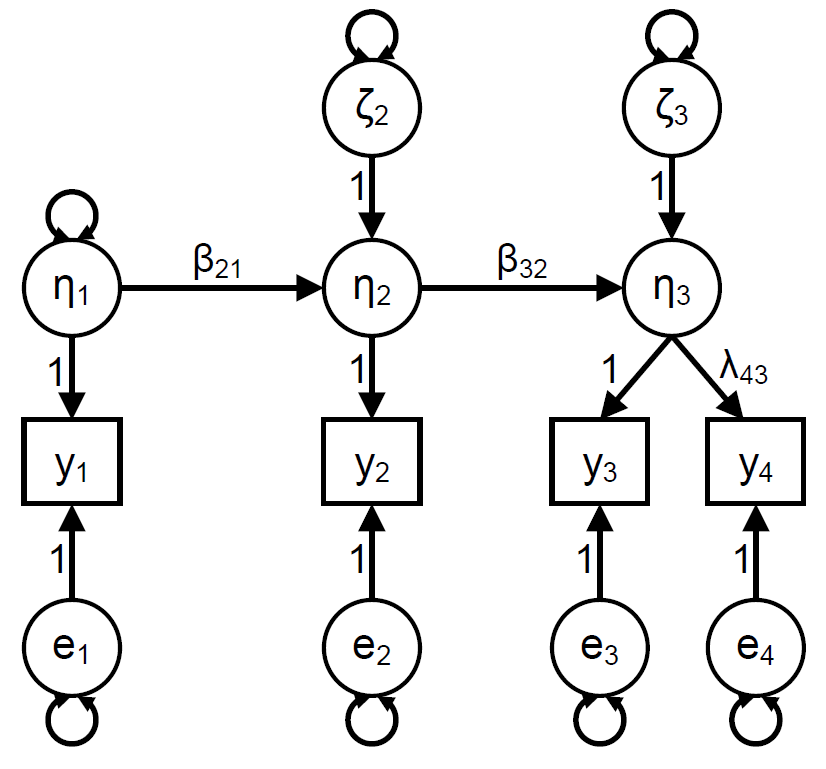
\includegraphics[width=4.16667in,height=\textheight]{Simplex-adjusted.png}
\caption{Adjusted quasi-simplex model.}
\end{figure}

Click to show answers

At each occasion there is a latent variable which represents Life Satisfaction. At the first two occasions there was only a single indicator of this latent variable, but at the third occasion there were two indicators.

\hypertarget{exercise-h}{%
\subsection{Exercise H}\label{exercise-h}}

How many \emph{df} does this model have? Note that we keep the constraint on the variances of the measurement errors.

Click to show answers

There are \(\frac{4*5}{2} = 10\) unique elements in S. We freely estimate:

\begin{itemize}
\tightlist
\item
  1 constrained residual variances at measurement level
\item
  1 factor variance
\item
  2 residual factor variances
\item
  2 regression parameters
\item
  1 factor loading
\item
  7 parameters in total.
\end{itemize}

Therefore, we have \(10 - 7 = 3\) \emph{df}.

\hypertarget{exercise-i}{%
\subsection{Exercise I}\label{exercise-i}}

Are these two models nested? If so, how? If not, why not, and how could we compare them?

Click to show answers

Yes, they are nested: this model is a special case of the previous model, as it is based on having \texttt{ETA3} and \texttt{ETA4} from the previous model now being a single latent variable. That is, we can constrain the residual variance of \texttt{ETA4} to zero to get the alternative model. This gives us 1 \emph{df} for the difference.

\hypertarget{exercise-j}{%
\subsection{Exercise J}\label{exercise-j}}

Specify this model in Mplus and run it. Report on the model fit.

Click to show answers

See the Mplus input file \texttt{Excercise\ J.inp} for the model specification in Mplus. Apart from the \(\chi^{2}\)-test of model fit, the model fits well:

\begin{itemize}
\tightlist
\item
  \(\chi^{2} (3) = 27.37\), with \(p < .001\),
\item
  RMSEA = 0.069,
\item
  CFI = 0.987,
\item
  TLI = 0.973, and
\item
  SRMR = 0.039.
\end{itemize}

\hypertarget{exercise-k}{%
\subsection{Exercise K}\label{exercise-k}}

Compare the two models to each other. What can you conclude?

Click to show answers

Comparing both models using the \(\Delta \chi^{2}\)-test gives us \(27.37 – 13.29 = 14.0\) with 1 \emph{df} such that \(p < .001\). This implies that imposing the restriction is not tenable. You can calculate the \emph{p}-value of the \(\Delta \chi^{2}\) using the \texttt{pchisq()}-function in R (with the \texttt{lower.tail} argument set to \texttt{FALSE}), or \href{http://www.fourmilab.ch/rpkp/experiments/analysis/chiCalc.html}{an online tool}

Comparing the models using information criteria gives us AIC = 29593 and BIC = 29637 for the first model, and AIC = 29605 and BIC = 29643 for the second. In conclusion, all measures indicate the first model is better. However, the current model makes more theoretical sense, and the negative variance estimate in the first model is a problem. For these 2 reasons, we should prefer the current model.

\hypertarget{exercise-l}{%
\subsection{Exercise L}\label{exercise-l}}

Can you improve the second model in any way? Indicate which parameter you would add to your model, and what this parameter represents in substantive terms.

Click to show answers

You can get the modification indices by adding \texttt{MOD} to the \texttt{OUTPUT} command. Here, the suggested BY statements make no sense (later life satisfaction as an indicator of previous life satisfaction). With regards to the ON statement, only the suggested effect of \texttt{ETA3\ ON\ ETA1} makes sense as we then predict forwards in time. The WITH statement suggests adding a covariance between the residuals of \texttt{y3} and \texttt{y4}. If we add this covariance and look at the standardized results, we get a correlation. This correlation actually quite high: \(.522\) (SE = .044), \(p < .001\).

\hypertarget{exercise-m}{%
\subsection{Exercise M}\label{exercise-m}}

Run a model in which you include the \texttt{Y3\ WITH\ Y4} parameter. Where will this relationship end up in the model? Does it lead to a significant improvement? How would you interpret this additional parameter?

Click to show answers

See \texttt{Exercise\ M.inp} for the Mplus specification of this model. The \texttt{Y3\ WITH\ Y4} parameter is an additional covariance between the residuals of \texttt{y3} and \texttt{y4} (so not between \texttt{y3} and \texttt{y4} themselves). Model fit is quite good (except for the \(\chi^{2}\)-test of model fit):

\begin{itemize}
\tightlist
\item
  \(\chi^{2} (2) = 7.077\), \(p = .0291\),
\item
  RMSEA = 0.038,
\item
  CFI = 0.997,
\item
  TLI = 0.992, and
\item
  SRMR = 0.011.
\end{itemize}

To compare this model to the previous model, we can do a the \(\Delta \chi^{2}\)-test: \(27.37 – 7.08 = 20.29\), with 1 \emph{df} such that \(p < .001\), which implies that adding the covariance between the residuals leads to a significant improvement in model fit. This additional parameter implies that \texttt{y3} and \texttt{y4} have more in common with each other than what would be expected based on their common dependence on \texttt{ETA3}. Note that in the standardized results, the WITH statement can be interpreted as a correlation, and it is quite high: \(.522\) (SE = .044), \(p < .001\).

\hypertarget{clpm-ri-clpm}{%
\section{CLPM \& RI-CLPM}\label{clpm-ri-clpm}}

For the cross-lagged panel model (CLPM) and the random intercept cross-lagged panel model (RI-CLPM) we are going to analyze data that were reported in \href{10.1017/S0954579416000237}{Davies, Martin, Coe and Cummings (2016)}. The summary data (means, standard deviations and correlation matrix) are included in Davies.dat, and contains the means, standard deviations, and the correlation matrix. The number of observations is 232. There are 5 waves of data, taken when the child was 7, 8, 13, 14, and 15 years old. The order of the variables is:

\begin{itemize}
\tightlist
\item
  Child gender
\item
  Parental education
\item
  Interparental hostility (waves 1-5): composite score based on observational data and questionnaires, reflecting the degree of hostility between the parents
\item
  Interparental dysphoria (waves 1-5): based on composite score based on observational data and questionnaires, reflecting the degree of dysphoria
\item
  Child/adolescent insecurity in the relationship with the parents (waves 1-5)
\item
  Psychological problems (waves 1-5): based on the subscales anxious/depressed, withdrawal, aggressive behaviors, and delinquency scales of the Child Behavior Checklist (CBCL), filled out by both parents.
\end{itemize}

Here we will focus on \emph{Interparental dysphoria} and \emph{Psychological problems} of the child. The DATA and VARIABLE commands should be:

\begin{verbatim}
DATA: 
  TYPE = MEANS STDEVIATIONS CORRELATION;
  FILE = Davies.dat;
  NOBSERVATIONS = 232;

VARIABLE: 
  NAMES = ChildGen ParentEd
  Hos1 Hos2 Hos3 Hos4 Hos5 Dys1 Dys2 Dys3 Dys4 Dys5
  Ins1 Ins2 Ins3 Ins4 Ins5 PsPr1 PsPr2 PsPr3 PsPr4 PsPr5;
  USEVARIABLES = Dys1-Dys5 PsPr1-PsPr5;
\end{verbatim}

\hypertarget{exercise-a-1}{%
\subsection{Exercise A}\label{exercise-a-1}}

How many sample statistics are there for this data set (focusing on the 5 measures of dysphoria and the 5 measures of psychological problems?

Click to show answers

There are 10 observed variables such that there are \(\frac{10*11}{2} = 55\) unique elements in the observed covariance matrix S, and 10 observed means in M. Therefore, there are 65 sample statistics in total.

\hypertarget{exercise-b-1}{%
\subsection{Exercise B}\label{exercise-b-1}}

We begin with an RI-CLPM (see slide 53). For now, do not impose any constraints on the parameters across time. Draw the model, and indicate which parameters will be estimated freely. How many parameters will be estimated in total? So how many \emph{df} are there?

Click to show answers

In the RI-CLPM we estimate:

\begin{itemize}
\tightlist
\item
  2 variances for the random intercepts,
\item
  1 covariance between the random intercepts,
\item
  2 variances for the within-person centered variables at wave 1,
\item
  1 covariance between the within-person centered variables at wave 1,
\item
  8 residual variances (for the dynamic errors of both variables at wave 2-5),
\item
  4 covariances between the residuals (for the dynamics errors at waves 2-5),
\item
  16 lagged parameters (4 for each interval), and
\item
  10 means.
\end{itemize}

In total, we estimate 44 parameters such that we have \(65 - 44 = 21\) \emph{df}.

\hypertarget{exercise-c-1}{%
\subsection{Exercise C}\label{exercise-c-1}}

Run the model. Check whether the number of \emph{df} is correct. Also look at the TECH1 output, to see if you understand where the free parameters are. What is the model fit?

Click to show answers

The input for this model is in \texttt{RICLPM.inp}. The model means are estimated in the \(\nu\)-matrix, no parameters are estimated in the \(\theta\)-matrix (measurement error variances), \(\lambda\)-matrix (factor loadings), or \(\alpha\)-matrix (means/intercepts of the latent variables). The variances and covariance of the random intercepts, the within-person centered variables at wave 1, and the dynamic errors at subsequent waves are all estimated in the \(\psi\)-matrix. The lagged regression coefficients are estimated in \(\beta\).

Apart from the \(\chi^{2}\)-test of model, all fit indices indicate at least acceptable fit.

\begin{itemize}
\tightlist
\item
  \(\chi^{2} (21) = 41.451\), \(p = .005\),
\item
  RMSEA = 0.065,
\item
  CFI = 0.979,
\item
  TLI = 0.956, and
\item
  SRMR = 0.029.
\end{itemize}

\hypertarget{exercise-d-1}{%
\subsection{Exercise D}\label{exercise-d-1}}

Include the significant standardized parameter estimates for the covariances (i.e., the WITH statements) and the lagged regression parameters (i.e., the ON statements) in the figure below. Indicate which part of the model is considered the between-person part, and which part is the within-person part.

\begin{figure}
\centering
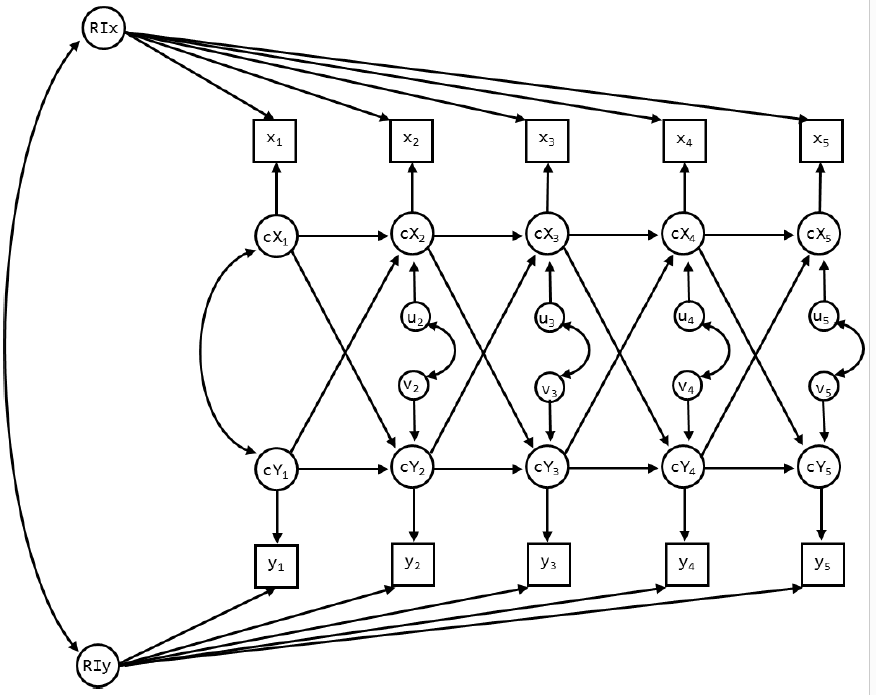
\includegraphics[width=5.20833in,height=\textheight]{figures/RICLPM-5waves.png}
\caption{The bivariate random-intercept cross-lagged panel model with 5 repeated measures (waves).}
\end{figure}

\hypertarget{exercise-e-1}{%
\subsection{Exercise E}\label{exercise-e-1}}

Omit the random intercepts. How many parameters and \emph{df} does this model have? What is the model fit?

Click to show answers

The input for this model is \texttt{CLPMasRICLPM.inp}. The model has three parameters less (and thus 3 \emph{df} more) than the previous model: 2 variances and the covariance for the random intercepts.

The model fit indices show that this model does not fit well:

\begin{itemize}
\tightlist
\item
  \(\chi^{2} (24) = 73.374\), \(p < .001\),
\item
  RMSEA = 0.094,
\item
  CFI = 0.950,
\item
  TLI = 0.907, and
\item
  SRMR = 0.061.
\end{itemize}

\hypertarget{exercise-f-1}{%
\subsection{Exercise F}\label{exercise-f-1}}

Specify the CLPM and run this model. Compare it to the previous two models. How are these models related?

Click to show answers

The input for this model is in \texttt{CLPM.inp}. This model is statistically identical to the previous model; these are different parameterizations of the same model. The model fit is therefore also exactly the same. Hence, this model is a special case of the RI-CLPM.

Comparing the two models using a chi-square difference test gives: \(\Delta \chi^{2} = 73.37 - 41.45 = 31.92\) with \(24 – 21 = 3\) \emph{df}, \(p < .001\). Hence, the random intercepts should not be omitted; put differently, there are stable, trait-like difference between families in the two variables (parental dysphoria and psychological problems).

However, when constraints are placed on the bound of the parameter space (which is the case here, fixing a variance to 0 is its absolute minimum value), we should actually use the chi-bar-square test (\(\bar{\chi}^{2}\)-test; Stoel et al.~2006). The traditional \(\Delta \chi^{2}\)-test does not take into account that variances can only be positive and is therefore conservative. This means that if it is significant, we are certain that the correct test (i.e., the \(\bar{\chi}^{2}\) test) would also be significant. On the other hand, when the usual chi‐square test is not significant, we do not know anything about the result of the correct test (it can be significant or not significant).

If you are working in R with the lavaan-package, you can find more information about the \(\bar{\chi}^{2}\)-test at \href{https://jeroendmulder.github.io/RI-CLPM/lavaan.html\#(bar\%7Bchi\%7D\%5E\%7B2\%7D)-test}{jeroendmulder.github.io/RI-CLPM/lavaan.html\#(bar\{chi\}\^{}\{2\})-test}. For Mplus users, there is a \href{https://www.uu.nl/staff/RMKuiper/Websites\%20\%2F\%20Shiny\%20apps}{Shiny app by Rebecca Kuiper} available as well.

\hypertarget{exercise-g-1}{%
\subsection{Exercise G}\label{exercise-g-1}}

Include the significant standardized parameter estimates for the covariances and the lagged regression parameters in the figure below.

\begin{figure}
\centering
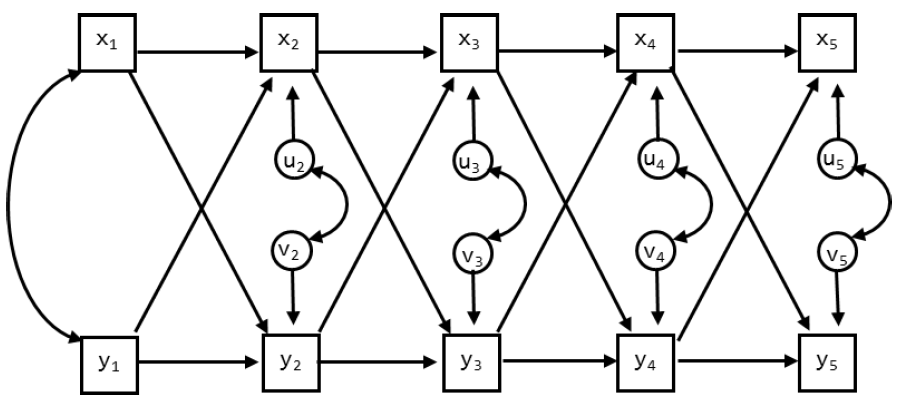
\includegraphics[width=5.20833in,height=\textheight]{CLPM-5waves.png}
\caption{The bivariate cross-lagged panel model with 5 repeated measures (waves).}
\end{figure}

\hypertarget{exercise-h-1}{%
\subsection{Exercise H}\label{exercise-h-1}}

Discuss how the model results differ.

Click to show answers

\textbf{Cross-lagged relationships}
In the RI-CLPM none of the cross-lagged parameters are significant. In contrast, in the CLPM there is a positive relationship from \texttt{PsPr1} to \texttt{Dys2}. This implies that higher levels of children's psychological problems at age 7 are followed by higher levels of interparental dysphoria at age 8. Moreover, from age 14 to 15 both cross-lagged parameters are significant and positive, indicating that psychological problems are followed by increases in interparental dysphoria, but also that increased interparental dysphoria is followed by an increase in psychological problems for the adolescent.

\textbf{Autoregressive parameters}
The autoregressive parameters in the RI-CLPM are lower, and have larger SE's, such that fewer reach significance. This is expected as within-person stability is now captures in the random intercepts, rather than in the autoregressive effects in the CLPM.

\textbf{Correlations}
In the CLPM only the residual correlation at wave 2 is significant; it is negative, indicating that external effects tend to have an opposite effect on these two processes; increases in Dysphoria are accompanied by decreases in psychological problems and vice versa. In the RI-CLPM, the within-person correlation at wave 1 is not significantly different from zero; however, at waves 2, 3 and 4 the correlations between the residuals is significant and negative. At wave 5 the residual variance is not significant.

In the RI-CLPM there is also the correlation between the random intercepts (i.e., the trait-like difference between families). This turns out to be a very substantial correlation of .63: Hence, in contrast to the results from the CLPM and the within-level results from the RI-CLPM, there is a strong positive relationship between trait-like levels of interparental dysphoria and trait-like levels of psychological problems.

\end{document}
